% Revisão OK 12/10
\chapter{Rotas do back-end}

A seguir são listadas e explicadas todas as rotas públicas do backend. As
rotas de administração são explicadas na seção "Interface de Administração".

\section{Rota raiz}

Página inicial, apresenta a lista de aeródromos para que o usuário escolha um. 
Internamente, por meio do ORM, é feita a seleção dos campos \texttt{AerodromeName},
\texttt{ICAO} e \texttt{City} dos aerodromos com isPublished como verdadeiro e o
 resultado é posto em uma lista de tuplas que é enviada para o template.

Para um usuário logado também são mostrados os aeróromos não publicados.

Exemplo do resultado enviado à ferramenta de template:

\lstinputlisting[label=resp:root, title={Resposta da root}, caption={Resposta da root}, language=Python]{code/resp-root.json}


\section{Rota: /info/\{ICAO\}}

Retorna informações do aerodrómo e seu metar decodificado. A seguir um exemplo
de resultado enviado ao Jinja2.

\lstinputlisting[label=resp:root, title={Resposta da rota info}, caption={Resposta da rota info}, language=Python]{code/resp-info.json}


\section{Rota: /history/\{ICAO\}}
É uma página estatica com os gráficos históricos para os doze últimos METARs.
Mais informações do capítulo "Plotagem do METAR Histórico".


\section{Rota: /taf/\{ICAO\}}
Retorna o próximo TAF válido para este aeródromo com a explicação de cada item.

Exemplo do resultado enviado à ferramenta de template para o aeroporto do Galeão.

\lstinputlisting[label=resp:root, title={Resposta da rota taf}, caption={Resposta da rota tag}, language=Python]{code/resp-taf.json}


Perceba que os grupos TEMPO e BECMG são agrupados para que no front-end o usuário 
possa exibir ou ocultar cada grupo. Conforme mostra a imagem abaixo.


\begin{figure}[ht]
    \begin{center}
    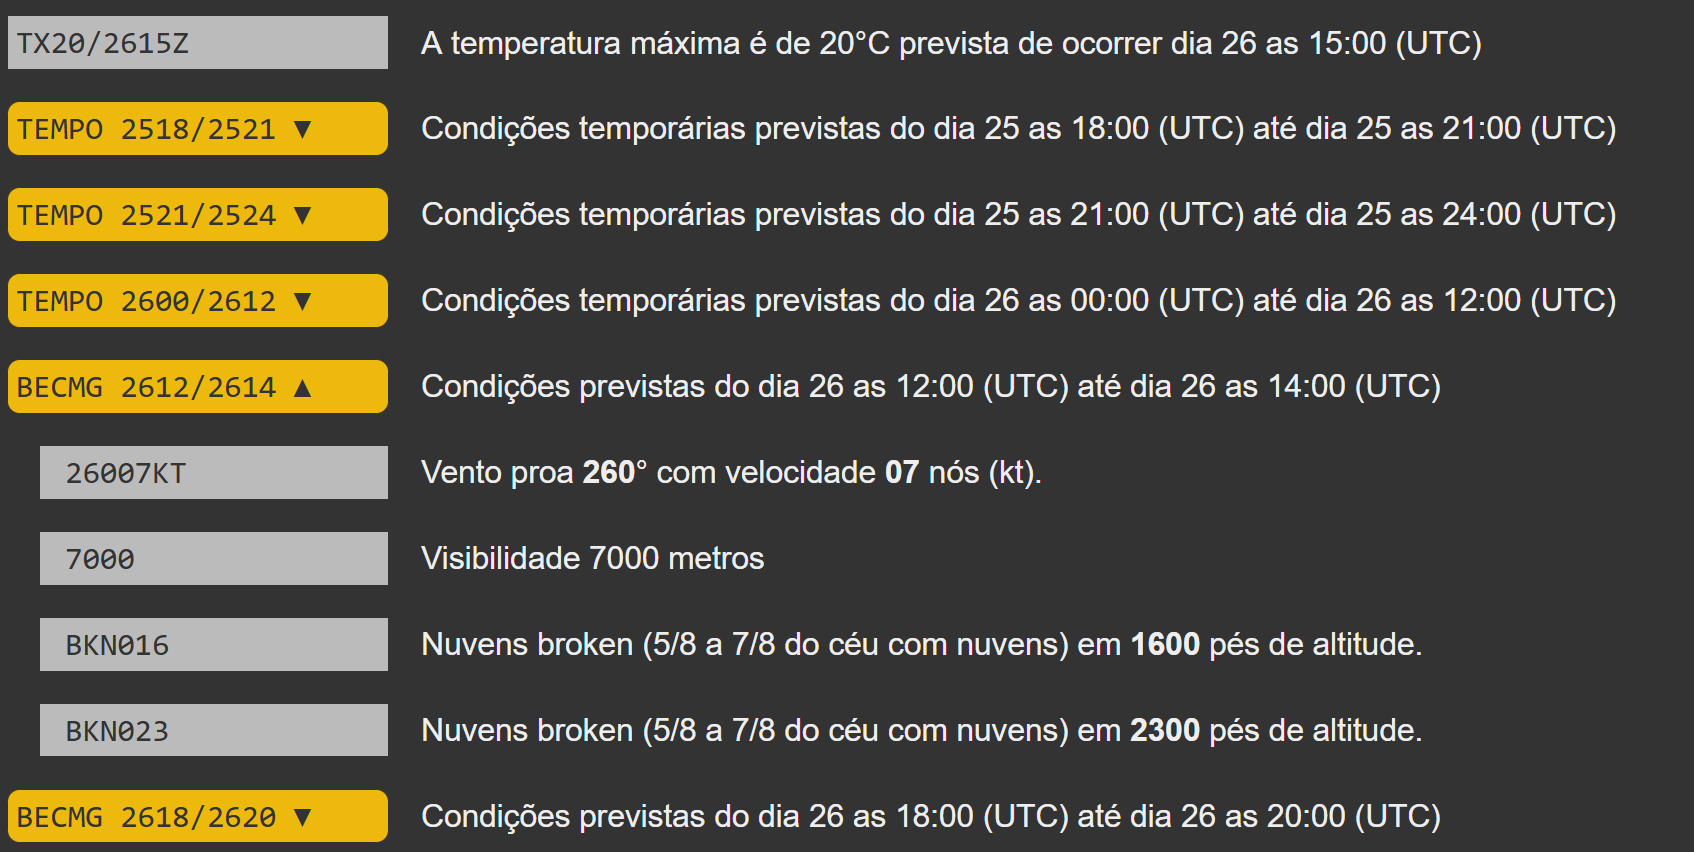
\includegraphics[width=400pt]{img/BECMG-exibido.png}
    \caption{Grupo BECMG exibido}
    \label{fig:becmg-exibido}
    \end{center}
\end{figure}


